% answers.tex —— 2015 年·陕西卷·文史类 · 参考答案与详细解析片段
% 由 tools/generate_projects.py 依来源总账自 2015/2015_数学真题_陕西文_试题.md + 2015/2015_数学真题_陕西文_解析正文.md + 2015/2015_数学真题_陕西文_答案要点.md 生成，勿手改（改源 MD 后重跑）


\gkpart{一、选择题（第 1—12 题）}

\begin{answer}
\gksolhead{1}{}

\textbf{题目}：

设集合 $M=\{x\mid x^{2}=x\}$，$N=\{x\mid \lg x\le 0\}$，则 $M\cup N=$（　）。

（A）$[0,1]$；（B）$(0,1]$；（C）$[0,1)$；（D）$(-\infty,1]$。

\Needspace{4\baselineskip}
\textbf{解析}

由 $x^{2}=x$ 得 $x=0$ 或 $x=1$，故 $M=\{0,1\}$。

由 $\lg x\le 0=\lg 1$ 且对数有意义得 $0<x\le 1$，故 $N=(0,1]$。

\Needspace{5\baselineskip}
于是

\nopagebreak[4]
\[
M\cup N=\{0,1\}\cup(0,1]=[0,1].
\]

\gkanswer{答案：A。}

\end{answer}
\begin{answer}
\gksolhead{2}{}

\textbf{题目}：

某中学初中部共有 $110$ 名教师，高中部共有 $150$ 名教师，其性别比例如图所示，则该校女教师的人数为（　）。
\nopagebreak[4]
\begin{center}% 2015 年陕西卷（文史类）第 2 题：教师性别比例饼图（依固定扫描页重绘，只画拓扑与标号，不按比例）
\begin{tikzpicture}[scale=1.0]
  % 左图：初中部，女 70%
  \fill[gray!30] (0,0) -- (35:1.3) arc (35:287:1.3) -- cycle;
  \draw (0,0) circle (1.3);
  \draw (0,0) -- (35:1.3);
  \draw (0,0) -- (287:1.3);
  \node at (170:0.72) {70\%};
  \node at (215:0.72) {女};
  \node at (-10:0.62) {男};
  \node at (0,-1.72) {（初中部）};
  % 右图：高中部，男 60%
  \begin{scope}[xshift=4.2cm]
    \fill[gray!30] (0,0) -- (105:1.3) arc (105:249:1.3) -- cycle;
    \draw (0,0) circle (1.3);
    \draw (0,0) -- (105:1.3);
    \draw (0,0) -- (249:1.3);
    \node at (177:0.72) {女};
    \node at (30:0.90) {60\%};
    \node at (-35:0.55) {男};
    \node at (0,-1.72) {（高中部）};
  \end{scope}
\end{tikzpicture}
\end{center}
\nopagebreak[4]
（A）$93$；（B）$123$；（C）$137$；（D）$167$。

\Needspace{4\baselineskip}
\textbf{解析}

\Needspace{5\baselineskip}
初中部女教师人数为

\nopagebreak[4]
\[
110\times 70\%=77.
\]

\Needspace{5\baselineskip}
高中部男教师占 $60\%$，故女教师占 $40\%$，人数为

\nopagebreak[4]
\[
150\times 40\%=60.
\]

全校女教师人数为 $77+60=137$。

\gkanswer{答案：C。}

\end{answer}
\begin{answer}
\gksolhead{3}{}

\textbf{题目}：

已知抛物线 $y^{2}=2px$（$p>0$）的准线经过点 $(-1,1)$，则该抛物线焦点坐标为（　）。

（A）$(-1,0)$；（B）$(1,0)$；（C）$(0,-1)$；（D）$(0,1)$。

\Needspace{4\baselineskip}
\textbf{解析}

\Needspace{5\baselineskip}
抛物线 $y^{2}=2px$（$p>0$）的准线为 $x=-\dfrac{p}{2}$。它经过点 $(-1,1)$，而该点的纵坐标不影响准线方程，故

\nopagebreak[4]
\[
-\frac{p}{2}=-1,\qquad p=2.
\]

焦点为 $\left(\dfrac{p}{2},0\right)=(1,0)$。

\gkanswer{答案：B。}

\end{answer}
\begin{answer}
\gksolhead{4}{}

\textbf{题目}：

设 $f(x)=\begin{cases}1-\sqrt{x}, & x\ge 0,\\[2pt] 2^{x}, & x<0,\end{cases}$ 则 $f(f(-2))=$（　）。

（A）$-1$；（B）$\dfrac{1}{4}$；（C）$\dfrac{1}{2}$；（D）$\dfrac{3}{2}$。

\Needspace{4\baselineskip}
\textbf{解析}

\Needspace{5\baselineskip}
因 $-2<0$，先代入第二段：

\nopagebreak[4]
\[
f(-2)=2^{-2}=\frac{1}{4}.
\]

\Needspace{5\baselineskip}
$\dfrac{1}{4}\ge 0$，再代入第一段：

\nopagebreak[4]
\[
f\left(\frac{1}{4}\right)=1-\sqrt{\frac{1}{4}}=1-\frac{1}{2}=\frac{1}{2}.
\]

\gkanswer{答案：C。}

\end{answer}
\begin{answer}
\gksolhead{5}{}

\textbf{题目}：

一个几何体的三视图如图所示，则该几何体的表面积为（　）。
\nopagebreak[4]
\begin{center}% 2015 年陕西卷（文史类）第 5 题：三视图（依固定扫描页重绘，只画拓扑与标号，不按比例）
\begin{tikzpicture}[>=stealth,scale=1.0]
  % 正视图：边长 2 的正方形
  \draw (0,0) rectangle (2,2);
  \draw[<->] (0,-0.3)--(2,-0.3);
  \node at (1,-0.62) {$2$};
  \draw[<->] (2.3,0)--(2.3,2);
  \node at (2.68,1) {$2$};
  \node at (1,-1.05) {正视图};
  % 左视图：宽 1、高 2 的长方形（扫描页未标尺寸）
  \draw (4.0,0) rectangle (5.0,2);
  \node at (4.5,-1.05) {左视图};
  % 俯视图：宽 2、高 1 的半圆
  \draw (0,-2.4)--(2,-2.4);
  \draw (0,-2.4) arc (180:0:1);
  \draw[<->] (2.3,-2.4)--(2.3,-1.4);
  \node at (2.68,-1.9) {$1$};
  \node at (1,-3.9) {俯视图};
\end{tikzpicture}
\end{center}
\nopagebreak[4]
（A）$3\pi$；（B）$4\pi$；（C）$2\pi+4$；（D）$3\pi+4$。

\Needspace{4\baselineskip}
\textbf{解析}

由三视图可知该几何体是底面为半圆、高为 $2$ 的半圆柱，底面半圆半径为 $1$。

表面由三部分组成：曲侧面（半个圆柱侧面）面积为 $\pi r h=2\pi$；两个半圆底面合起来是一个整圆，面积为 $\pi r^{2}=\pi$；正视图所对的矩形平面面积为 $2r\cdot h=4$。

\Needspace{5\baselineskip}
故表面积

\nopagebreak[4]
\[
S=2\pi+\pi+4=3\pi+4.
\]

\gkanswer{答案：D。}

\end{answer}
\begin{answer}
\gksolhead{6}{}

\textbf{题目}：

“$\sin\alpha=\cos\alpha$”是“$\cos 2\alpha=0$”的（　）。

（A）充分不必要条件；（B）必要不充分条件；（C）充分必要条件；（D）既不充分也不必要条件。

\Needspace{4\baselineskip}
\textbf{解析}

\Needspace{5\baselineskip}
若 $\sin\alpha=\cos\alpha$，则 $\sin^{2}\alpha=\cos^{2}\alpha$，从而

\nopagebreak[4]
\[
\cos 2\alpha=\cos^{2}\alpha-\sin^{2}\alpha=0.
\]

反之，若 $\cos 2\alpha=0$，只能得到 $\sin^{2}\alpha=\cos^{2}\alpha$，即 $\sin\alpha=\pm\cos\alpha$。取 $\alpha=\dfrac{3\pi}{4}$，则 $\cos 2\alpha=\cos\dfrac{3\pi}{2}=0$，但 $\sin\alpha=\dfrac{\sqrt{2}}{2}\ne-\dfrac{\sqrt{2}}{2}=\cos\alpha$。

所以是充分不必要条件。

\gkanswer{答案：A。}

\end{answer}
\begin{answer}
\gksolhead{7}{}

\textbf{题目}：

根据框图，当输入 $x$ 为 $6$ 时，输出的 $y=$（　）。
\nopagebreak[4]
\begin{center}% 2015 年陕西卷（文史类）第 7 题：程序框图（依固定扫描页重绘，只画拓扑与标号，不按比例）
\begin{tikzpicture}[>=stealth,scale=0.95]
  % 开始
  \draw[rounded corners=6pt] (-1.0,0.4) rectangle (1.0,-0.4);
  \node at (0,0) {开始};
  \draw[->] (0,-0.4)--(0,-1.0);
  % 输入 x
  \draw (-1.0,-1.0)--(1.2,-1.0)--(1.0,-1.8)--(-1.2,-1.8)--cycle;
  \node at (0,-1.4) {输入 $x$};
  \draw[->] (0,-1.8)--(0,-2.3);
  % 赋值 x = x - 3
  \draw (-1.3,-2.3) rectangle (1.3,-3.1);
  \node at (0,-2.7) {$x=x-3$};
  \draw[->] (0,-3.1)--(0,-3.7);
  % 判断 x >= 0
  \draw (-1.9,-4.4)--(0,-3.7)--(1.9,-4.4)--(0,-5.1)--cycle;
  \node at (0,-4.4) {$x\ge 0$};
  % 是：回到赋值框
  \draw[->] (1.9,-4.4)--(3.2,-4.4)--(3.2,-2.7)--(1.3,-2.7);
  \node at (2.35,-4.05) {是};
  % 否：向下
  \draw[->] (0,-5.1)--(0,-5.7);
  \node at (0.32,-5.4) {否};
  % y = x^2 + 1
  \draw (-1.4,-5.7) rectangle (1.4,-6.5);
  \node at (0,-6.1) {$y=x^{2}+1$};
  \draw[->] (0,-6.5)--(0,-7.1);
  % 输出 y
  \draw (-1.0,-7.1)--(1.2,-7.1)--(1.0,-7.9)--(-1.2,-7.9)--cycle;
  \node at (0,-7.5) {输出 $y$};
  \draw[->] (0,-7.9)--(0,-8.5);
  % 结束
  \draw[rounded corners=6pt] (-1.0,-8.5) rectangle (1.0,-9.3);
  \node at (0,-8.9) {结束};
\end{tikzpicture}
\end{center}
\nopagebreak[4]
（A）$1$；（B）$2$；（C）$5$；（D）$10$。

\Needspace{4\baselineskip}
\textbf{解析}

输入 $x=6$ 后反复执行 $x=x-3$：

第一次 $x=3\ge 0$，返回继续；第二次 $x=0\ge 0$，返回继续；第三次 $x=-3<0$，退出循环。

\Needspace{5\baselineskip}
此时

\nopagebreak[4]
\[
y=x^{2}+1=(-3)^{2}+1=10.
\]

\gkanswer{答案：D。}

\end{answer}
\begin{answer}
\gksolhead{8}{}

\textbf{题目}：

对任意向量 $\boldsymbol{a}$，$\boldsymbol{b}$，下列关系式中不恒成立的是（　）。

（A）$|\boldsymbol{a}\cdot\boldsymbol{b}|\le|\boldsymbol{a}||\boldsymbol{b}|$；（B）$|\boldsymbol{a}-\boldsymbol{b}|\le||\boldsymbol{a}|-|\boldsymbol{b}||$；（C）$(\boldsymbol{a}+\boldsymbol{b})^{2}=|\boldsymbol{a}+\boldsymbol{b}|^{2}$；（D）$(\boldsymbol{a}+\boldsymbol{b})\cdot(\boldsymbol{a}-\boldsymbol{b})=\boldsymbol{a}^{2}-\boldsymbol{b}^{2}$。

\Needspace{4\baselineskip}
\textbf{解析}

(A) 是数量积的基本不等式 $|\boldsymbol{a}\cdot\boldsymbol{b}|=|\boldsymbol{a}||\boldsymbol{b}||\cos\theta|\le|\boldsymbol{a}||\boldsymbol{b}|$。

(C) 对任意向量 $\boldsymbol{v}$ 有 $|\boldsymbol{v}|^{2}=\boldsymbol{v}\cdot\boldsymbol{v}=\boldsymbol{v}^{2}$，取 $\boldsymbol{v}=\boldsymbol{a}+\boldsymbol{b}$ 即得。

(D) 按分配律展开：$(\boldsymbol{a}+\boldsymbol{b})\cdot(\boldsymbol{a}-\boldsymbol{b})=\boldsymbol{a}^{2}-\boldsymbol{a}\cdot\boldsymbol{b}+\boldsymbol{b}\cdot\boldsymbol{a}-\boldsymbol{b}^{2}=\boldsymbol{a}^{2}-\boldsymbol{b}^{2}$。

(B) 不恒成立。取 $\boldsymbol{a}=(1,0)$，$\boldsymbol{b}=(-1,0)$，则 $\boldsymbol{a}-\boldsymbol{b}=(2,0)$，$|\boldsymbol{a}-\boldsymbol{b}|=2$，而 $||\boldsymbol{a}|-|\boldsymbol{b}||=0$，不等式不成立。

\gkanswer{答案：B。}

\end{answer}
\begin{answer}
\gksolhead{9}{}

\textbf{题目}：

设 $f(x)=x-\sin x$，则 $f(x)$（　）。

（A）既是奇函数又是减函数；（B）既是奇函数又是增函数；（C）是有零点的减函数；（D）是没有零点的奇函数。

\Needspace{4\baselineskip}
\textbf{解析}

\Needspace{5\baselineskip}
定义域为 $\mathbf{R}$，关于原点对称，且

\nopagebreak[4]
\[
f(-x)=-x-\sin(-x)=-x+\sin x=-(x-\sin x)=-f(x),
\]

故 $f$ 是奇函数。

\Needspace{5\baselineskip}
又

\nopagebreak[4]
\[
f'(x)=1-\cos x\ge 0,
\]

等号只在 $x=2k\pi$ 处成立，这些点孤立，故 $f$ 在 $\mathbf{R}$ 上严格单调递增。

所以 $f$ 既是奇函数又是增函数。

\gkanswer{答案：B。}

\end{answer}
\begin{answer}
\gksolhead{10}{}

\textbf{题目}：

设 $f(x)=\ln x$，$0<a<b$，若 $p=f\left(\sqrt{ab}\right)$，$q=f\left(\dfrac{a+b}{2}\right)$，$r=\dfrac{1}{2}(f(a)+f(b))$，则下列关系式中正确的是（　）。

（A）$q=r<p$；（B）$q=r>p$；（C）$p=r<q$；（D）$p=r>q$。

\Needspace{4\baselineskip}
\textbf{解析}

\Needspace{5\baselineskip}
由对数运算

\nopagebreak[4]
\[
p=f\left(\sqrt{ab}\right)=\ln\sqrt{ab}=\frac{1}{2}(\ln a+\ln b)=\frac{1}{2}(f(a)+f(b))=r.
\]

\Needspace{5\baselineskip}
又 $0<a<b$，由均值不等式 $\sqrt{ab}<\dfrac{a+b}{2}$，而 $\ln x$ 在 $(0,+\infty)$ 上递增，故

\nopagebreak[4]
\[
p=\ln\sqrt{ab}<\ln\frac{a+b}{2}=q.
\]

所以 $p=r<q$。

\gkanswer{答案：C。}

\end{answer}
\begin{answer}
\gksolhead{11}{}

\textbf{题目}：

某企业生产甲、乙两种产品均需用 $A$，$B$ 两种原料，已知生产 $1$ 吨每种产品所需原料及每天原料的可用限额如表所示．如果生产 $1$ 吨甲、乙产品可获利润分别为 $3$ 万元、$4$ 万元，则该企业每天可获得最大利润为（　）。

\begin{center}
\begin{tabular}{llll}
\toprule
 & 甲 & 乙 & 原料限额 \\
\midrule
$A$（吨） & $3$ & $2$ & $12$ \\
$B$（吨） & $1$ & $2$ & $8$ \\
\bottomrule
\end{tabular}
\end{center}

（A）$12$ 万元；（B）$16$ 万元；（C）$17$ 万元；（D）$18$ 万元。

\Needspace{4\baselineskip}
\textbf{解析}

\Needspace{5\baselineskip}
设每天生产甲、乙产品分别为 $x$，$y$ 吨，利润为 $z=3x+4y$，约束为

\nopagebreak[4]
\[
\begin{cases}
3x+2y\le 12,\\
x+2y\le 8,\\
x\ge 0,\ y\ge 0.
\end{cases}
\]

可行域的顶点为 $(0,0)$，$(4,0)$，$(0,4)$，以及两直线交点 $(2,3)$。

逐点计算：$z(0,0)=0$，$z(4,0)=12$，$z(0,4)=16$，$z(2,3)=6+12=18$。

故最大利润为 $18$ 万元。

\gkanswer{答案：D。}

\end{answer}
\begin{answer}
\gksolhead{12}{}

\textbf{题目}：

设复数 $z=(x-1)+y\mathrm{i}$（$x,y\in\mathbf{R}$），若 $|z|\le 1$，则 $y\ge x$ 的概率为（　）。

（A）$\dfrac{3}{4}+\dfrac{1}{2\pi}$；（B）$\dfrac{1}{2}+\dfrac{1}{\pi}$；（C）$\dfrac{1}{4}-\dfrac{1}{2\pi}$；（D）$\dfrac{1}{2}-\dfrac{1}{\pi}$。

\Needspace{4\baselineskip}
\textbf{解析}

$|z|\le 1$ 即 $(x-1)^{2}+y^{2}\le 1$，是圆心为 $(1,0)$、半径为 $1$ 的圆盘，面积为 $\pi$。

\Needspace{5\baselineskip}
所求为圆盘内满足 $y\ge x$ 的部分。圆心到直线 $x-y=0$ 的距离为

\nopagebreak[4]
\[
d=\frac{|1-0|}{\sqrt{2}}=\frac{1}{\sqrt{2}}<1,
\]

\Needspace{5\baselineskip}
故该部分是一个弓形，其面积为

\nopagebreak[4]
\[
S=\arccos d-d\sqrt{1-d^{2}}=\arccos\frac{1}{\sqrt{2}}-\frac{1}{\sqrt{2}}\cdot\frac{1}{\sqrt{2}}=\frac{\pi}{4}-\frac{1}{2}.
\]

\Needspace{5\baselineskip}
所求概率为

\nopagebreak[4]
\[
P=\frac{S}{\pi}=\frac{1}{4}-\frac{1}{2\pi}.
\]

\gkanswer{答案：C。}

\end{answer}
\gkpart{二、填空题（第 13—16 题）}

\begin{answer}
\gksolhead{13}{}

\textbf{题目}：

中位数为 $1010$ 的一组数构成等差数列，其末项为 $2015$，则该数列的首项为 \gkblank{}。

\Needspace{4\baselineskip}
\textbf{解析}

\Needspace{5\baselineskip}
设该等差数列为 $a_{1},a_{2},\cdots,a_{n}$。等差数列的中位数等于首项与末项的算术平均（项数为奇数时是中间项，为偶数时是中间两项的平均，两种情形都等于 $\dfrac{a_{1}+a_{n}}{2}$），故

\nopagebreak[4]
\[
\frac{a_{1}+2015}{2}=1010,
\]

\Needspace{5\baselineskip}
解得

\nopagebreak[4]
\[
a_{1}=2020-2015=5.
\]

\gkanswer{答案：$5$。}

\end{answer}
\begin{answer}
\gksolhead{14}{}

\textbf{题目}：

如图，某港口一天 $6$ 时到 $18$ 时的水深变化曲线近似满足函数 $y=3\sin\left(\dfrac{\pi}{6}x+\varphi\right)+k$．据此函数可知，这段时间水深（单位：$\mathrm{m}$）的最大值为 \gkblank{}。
\nopagebreak[4]
\begin{center}% 2015 年陕西卷（文史类）第 14 题：水深随时间变化的曲线（依固定扫描页重绘，只画拓扑与标号，不按比例）
\begin{tikzpicture}[>=stealth,scale=1.0,xscale=0.55,yscale=0.62]
  % 坐标轴
  \draw[->] (0,0)--(7.2,0) node[above right] {时间/t};
  \draw[->] (0,-0.5)--(0,4.0) node[above right] {水深/m};
  \node[below left] at (0,0) {$O$};
  \node[left] at (0,1.0) {$2$};
  % 最低水位的虚线
  \draw[dashed] (0,1.0)--(2.82,1.0);
  % 曲线：最小值 2，最大值 8（示意）
  \draw[thick,domain=1.9:5.6,samples=120] plot (\x,{2.5-1.5*cos(180*(\x-2.82)/1.85)});
  % 时刻刻度
  \draw (1.9,0.06)--(1.9,-0.06);
  \node[below] at (1.9,0) {$6$};
  \draw (5.6,0.06)--(5.6,-0.06);
  \node[below] at (5.6,0) {$18$};
\end{tikzpicture}
\end{center}
\nopagebreak[4]
\Needspace{4\baselineskip}
\textbf{解析}

\Needspace{5\baselineskip}
设 $y=3\sin\left(\dfrac{\pi}{6}x+\varphi\right)+k$。正弦值的范围为 $[-1,1]$，故

\nopagebreak[4]
\[
y_{\min}=k-3,\qquad y_{\max}=k+3.
\]

图中曲线的最低点对应水深 $2\ \mathrm{m}$，即 $k-3=2$，得 $k=5$。

\Needspace{5\baselineskip}
所以最大水深为

\nopagebreak[4]
\[
k+3=8\ (\mathrm{m}).
\]

\gkanswer{答案：$8$。}

\end{answer}
\begin{answer}
\gksolhead{15}{}

\textbf{题目}：

函数 $y=x\mathrm{e}^{x}$ 在其极值点处的切线方程为 \gkblank{}。

\Needspace{4\baselineskip}
\textbf{解析}

\nopagebreak[4]
\[
y'=\mathrm{e}^{x}+x\mathrm{e}^{x}=(1+x)\mathrm{e}^{x}.
\]

\Needspace{5\baselineskip}
令 $y'=0$ 得 $x=-1$，这是唯一的极值点。此时

\nopagebreak[4]
\[
y\Big|_{x=-1}=-1\cdot \mathrm{e}^{-1}=-\frac{1}{\mathrm{e}}.
\]

\Needspace{5\baselineskip}
极值点处切线斜率为 $0$，故切线方程为

\nopagebreak[4]
\[
y=-\frac{1}{\mathrm{e}}.
\]

\gkanswer{答案：$y=-\dfrac{1}{\mathrm{e}}$。}

\end{answer}
\begin{answer}
\gksolhead{16}{}

\textbf{题目}：

\Needspace{5\baselineskip}
观察下列等式：

\nopagebreak[4]
\[
\begin{aligned}
1-\frac{1}{2}&=\frac{1}{2},\\
1-\frac{1}{2}+\frac{1}{3}-\frac{1}{4}&=\frac{1}{3}+\frac{1}{4},\\
1-\frac{1}{2}+\frac{1}{3}-\frac{1}{4}+\frac{1}{5}-\frac{1}{6}&=\frac{1}{4}+\frac{1}{5}+\frac{1}{6},\\
&\cdots\cdots,
\end{aligned}
\]

据此规律，第 $n$ 个等式可为 \gkblank{}。

\Needspace{4\baselineskip}
\textbf{解析}

三个等式的左边都是 $1-\dfrac{1}{2}+\dfrac{1}{3}-\cdots$ 的交错和，右边是从某个位置开始的一串倒数之和。

\Needspace{5\baselineskip}
第 $n$ 个等式左边共 $2n$ 项，末项为 $-\dfrac{1}{2n}$；右边从 $\dfrac{1}{n+1}$ 起，到 $\dfrac{1}{2n}$ 止，共 $n$ 项。即

\nopagebreak[4]
\[
1-\frac{1}{2}+\frac{1}{3}-\frac{1}{4}+\cdots+\frac{1}{2n-1}-\frac{1}{2n}=\frac{1}{n+1}+\frac{1}{n+2}+\cdots+\frac{1}{2n}.
\]

验证：$n=1$ 时左边 $1-\dfrac{1}{2}=\dfrac{1}{2}$，右边 $\dfrac{1}{2}$，成立。

\Needspace{5\baselineskip}
若第 $n$ 个等式成立，比较第 $n+1$ 个等式的两边与它的差。左边多出两项

\nopagebreak[4]
\[
\frac{1}{2n+1}-\frac{1}{2n+2};
\]

\Needspace{5\baselineskip}
右边由归纳假设，比原来的右边多出

\nopagebreak[4]
\[
-\frac{1}{n+1}+\frac{1}{2n+1}+\frac{1}{2n+2}.
\]

因 $-\dfrac{1}{n+1}+\dfrac{1}{2n+2}=-\dfrac{2}{2n+2}+\dfrac{1}{2n+2}=-\dfrac{1}{2n+2}$，上式等于 $\dfrac{1}{2n+1}-\dfrac{1}{2n+2}$，与左边多出的两项一致。故等式对一切正整数 $n$ 成立。

\gkanswer{答案：$1-\dfrac{1}{2}+\dfrac{1}{3}-\cdots+\dfrac{1}{2n-1}-\dfrac{1}{2n}=\dfrac{1}{n+1}+\dfrac{1}{n+2}+\cdots+\dfrac{1}{2n}$。}

\end{answer}
\gkpart{三、解答题（第 17—24 题）}

\begin{answer}
\gksolhead{17}{}

\textbf{题目}：

$\triangle ABC$ 的内角 $A$，$B$，$C$ 所对的边分别为 $a$，$b$，$c$．向量 $\boldsymbol{m}=(a,\sqrt{3}b)$ 与 $\boldsymbol{n}=(\cos A,\sin B)$ 平行．

（1） 求 $A$；

（2） 若 $a=\sqrt{7}$，$b=2$，求 $\triangle ABC$ 的面积．

\Needspace{4\baselineskip}
\textbf{解析}

\Needspace{5\baselineskip}
\textbf{（1）} 由 $\boldsymbol{m}\parallel\boldsymbol{n}$ 得

\nopagebreak[4]
\[
a\sin B-\sqrt{3}b\cos A=0.
\]

\Needspace{5\baselineskip}
由正弦定理 $\dfrac{a}{\sin A}=\dfrac{b}{\sin B}$，即 $a\sin B=b\sin A$，代入上式得

\nopagebreak[4]
\[
b\sin A=\sqrt{3}b\cos A.
\]

\Needspace{5\baselineskip}
因 $b>0$，故 $\tan A=\sqrt{3}$。又 $A\in(0,\pi)$，所以

\nopagebreak[4]
\[
A=\frac{\pi}{3}.
\]

\Needspace{5\baselineskip}
\textbf{（2）} 由余弦定理

\nopagebreak[4]
\[
a^{2}=b^{2}+c^{2}-2bc\cos A,
\]

\Needspace{5\baselineskip}
代入 $a=\sqrt{7}$，$b=2$，$A=\dfrac{\pi}{3}$ 得

\nopagebreak[4]
\[
7=4+c^{2}-2\cdot 2\cdot c\cdot\frac{1}{2},
\]

即 $c^{2}-2c-3=0$，解得 $c=3$（舍去 $c=-1$）。

\Needspace{5\baselineskip}
于是

\nopagebreak[4]
\[
S_{\triangle ABC}=\frac{1}{2}bc\sin A=\frac{1}{2}\cdot 2\cdot 3\cdot\frac{\sqrt{3}}{2}=\frac{3\sqrt{3}}{2}.
\]

\gkanswer{答案（1）：$A=\dfrac{\pi}{3}$。}

\gkanswer{答案（2）：$\triangle ABC$ 的面积为 $\dfrac{3\sqrt{3}}{2}$。}

\end{answer}
\begin{answer}
\gksolhead{18}{}

\textbf{题目}：

如图 1，在直角梯形 $ABCD$ 中，$AD\parallel BC$，$\angle BAD=\dfrac{\pi}{2}$，$AB=BC=\dfrac{1}{2}AD=a$，$E$ 是 $AD$ 的中点，$O$ 是 $AC$ 与 $BE$ 的交点．将 $\triangle ABE$ 沿 $BE$ 折起到图 2 中 $\triangle A_{1}BE$ 的位置，得到四棱锥 $A_{1}-BCDE$．

（1） 证明：$CD\perp$ 平面 $A_{1}OC$；

（2） 若平面 $A_{1}BE\perp$ 平面 $BCDE$，四棱锥 $A_{1}-BCDE$ 的体积为 $36\sqrt{2}$，求 $a$ 的值．
\nopagebreak[4]
\begin{center}% 2015 年陕西卷（文史类）第 18 题：折叠前的直角梯形与折叠后的四棱锥（依固定扫描页重绘，只画拓扑与标号，不按比例）
\begin{tikzpicture}[scale=0.85]
  % 图 1：直角梯形 ABCD，E 为 AD 中点，O 为 AC 与 BE 的交点
  \coordinate (A) at (0,2);
  \coordinate (B) at (0,0);
  \coordinate (C) at (2,0);
  \coordinate (D) at (3,2);
  \coordinate (E) at (1.5,2);
  \coordinate (O) at (0.75,1.25);
  \draw (A)--(D)--(C)--(B)--cycle;
  \draw (A)--(C);
  \draw (B)--(E);
  \node[above left] at (A) {$A$};
  \node[below left] at (B) {$B$};
  \node[below] at (C) {$C$};
  \node[above right] at (D) {$D$};
  \node[above] at (E) {$E$};
  \node[left] at (O) {$O$};
  \node at (1.5,-0.75) {图 1};
  % 图 2：折叠后所得四棱锥 A1-BCDE
  \begin{scope}[xshift=5.4cm]
    \coordinate (A1) at (0.9,3.0);
    \coordinate (B2) at (0.2,0.2);
    \coordinate (C2) at (2.2,0.2);
    \coordinate (D2) at (3.4,1.4);
    \coordinate (E2) at (1.4,1.4);
    \coordinate (O2) at (0.8,0.8);
    % 可见侧棱与底边：实线
    \draw (A1)--(B2);
    \draw (A1)--(C2);
    \draw (A1)--(D2);
    \draw (B2)--(C2);
    \draw (C2)--(D2);
    % 被遮挡的棱与辅助线：虚线
    \draw[dashed] (A1)--(E2);
    \draw[dashed] (D2)--(E2);
    \draw[dashed] (A1)--(O2);
    \draw[dashed] (B2)--(O2);
    \draw[dashed] (O2)--(E2);
    \draw[dashed] (O2)--(C2);
    \node[above] at (A1) {$A_{1}(A)$};
    \node[below left] at (B2) {$B$};
    \node[below] at (C2) {$C$};
    \node[right] at (D2) {$D$};
    \node[above left] at (E2) {$E$};
    \node[below] at (O2) {$O$};
    \node at (1.7,-0.75) {图 2};
  \end{scope}
\end{tikzpicture}
\end{center}
\nopagebreak[4]
\Needspace{4\baselineskip}
\textbf{解析}

\textbf{（1）} 由 $AB=BC=\dfrac{1}{2}AD=a$ 及 $E$ 为 $AD$ 中点得 $AE=ED=a$。又 $AD\parallel BC$，故 $AE\parallel BC$ 且 $AE=BC=a$，四边形 $ABCE$ 是平行四边形；由 $\angle BAD=\dfrac{\pi}{2}$ 知它是矩形，而 $AB=BC=a$，故 $ABCE$ 是边长为 $a$ 的正方形。

在正方形 $ABCE$ 中，对角线 $BE$ 与 $AC$ 互相垂直平分，交于点 $O$，故 $BE\perp AO$，$BE\perp OC$。

又 $BC\parallel ED$ 且 $BC=ED=a$，故 $BCDE$ 是平行四边形，从而 $CD\parallel BE$。

于是 $CD\perp AO$。

\Needspace{5\baselineskip}
折起后 $O$ 在折痕 $BE$ 上保持不动，$A$ 变为 $A_{1}$，而 $AO\perp BE$，所以 $A_{1}O$ 仍在过 $O$ 且垂直于 $BE$ 的平面内，依然有 $A_{1}O\perp BE$。由 $CD\parallel BE$ 得

\nopagebreak[4]
\[
CD\perp A_{1}O,\qquad CD\perp OC.
\]

\Needspace{5\baselineskip}
$A_{1}O$ 与 $OC$ 是平面 $A_{1}OC$ 内两条相交于 $O$ 的直线，故

\nopagebreak[4]
\[
CD\perp \text{平面 }A_{1}OC.
\]

\Needspace{5\baselineskip}
\textbf{（2）} 平面 $A_{1}BE\perp$ 平面 $BCDE$，交线为 $BE$。由（1）知 $A_{1}O\perp BE$，且 $A_{1}O\subset$ 平面 $A_{1}BE$，故

\nopagebreak[4]
\[
A_{1}O\perp \text{平面 }BCDE.
\]

\Needspace{5\baselineskip}
在正方形 $ABCE$ 中，

\nopagebreak[4]
\[
A_{1}O=AO=\frac{\sqrt{2}}{2}AB=\frac{\sqrt{2}}{2}a.
\]

\Needspace{5\baselineskip}
底面 $BCDE$ 是平行四边形，底 $BC=a$，高（$AD$ 与 $BC$ 之间的距离）为 $a$，故

\nopagebreak[4]
\[
S_{BCDE}=a^{2}.
\]

\Needspace{5\baselineskip}
四棱锥体积

\nopagebreak[4]
\[
V=\frac{1}{3}S_{BCDE}\cdot A_{1}O=\frac{1}{3}a^{2}\cdot\frac{\sqrt{2}}{2}a=\frac{\sqrt{2}}{6}a^{3}.
\]

\Needspace{5\baselineskip}
由 $\dfrac{\sqrt{2}}{6}a^{3}=36\sqrt{2}$ 得 $a^{3}=216$，故

\nopagebreak[4]
\[
a=6.
\]

\gkanswer{答案（1）：证明见解析。}

\gkanswer{答案（2）：$a=6$。}

\end{answer}
\begin{answer}
\gksolhead{19}{}

\textbf{题目}：

随机抽取一个年份，对西安市该年 $4$ 月份的天气情况进行统计，结果如下：

\begin{center}
\begingroup\setlength{\tabcolsep}{4pt}
\begin{tabular}{lllllllllll}
\toprule
日期 & 1 & 2 & 3 & 4 & 5 & 6 & 7 & 8 & 9 & 10 \\
\midrule
天气 & 晴 & 雨 & 阴 & 阴 & 阴 & 雨 & 阴 & 晴 & 晴 & 晴 \\
日期 & 11 & 12 & 13 & 14 & 15 & 16 & 17 & 18 & 19 & 20 \\
天气 & 阴 & 晴 & 晴 & 晴 & 晴 & 晴 & 阴 & 雨 & 阴 & 阴 \\
日期 & 21 & 22 & 23 & 24 & 25 & 26 & 27 & 28 & 29 & 30 \\
天气 & 晴 & 阴 & 晴 & 晴 & 晴 & 阴 & 晴 & 晴 & 晴 & 雨 \\
\bottomrule
\end{tabular}
\endgroup
\end{center}

（1） 在 $4$ 月份任取一天，估计西安市在该天不下雨的概率；

（2） 西安市某学校拟从 $4$ 月份的一个晴天开始举行连续 $2$ 天的运动会，估计运动会期间不下雨的概率．

\Needspace{4\baselineskip}
\textbf{解析}

\textbf{（1）} 4 月份共 $30$ 天，统计表中不下雨（晴或阴）的天数为 $30-4=26$（下雨的是 2、6、18、30 日，共 $4$ 天）。

\Needspace{5\baselineskip}
用频率估计概率：

\nopagebreak[4]
\[
P=\frac{26}{30}=\frac{13}{15}.
\]

\textbf{（2）} 晴天共有 $16$ 天：1、8、9、10、12、13、14、15、16、21、23、24、25、27、28、29 日。

运动会从某个晴天开始、连续 $2$ 天，要求第 $2$ 天也不下雨（阴天不算下雨）。逐一检查第 $2$ 天：

1 日次日下雨；8、9 日次日为晴；10 日次日为阴；12、13、14、15 日次日为晴；16 日次日为阴；21 日次日为阴；23、24 日次日为晴；25 日次日为阴；27、28 日次日为晴；29 日次日下雨。

次日不下雨的起点共 $14$ 个；只有 $1$ 日（次日 $2$ 日雨）与 $29$ 日（次日 $30$ 日雨）不满足，其余含次日为阴的 $10$、$16$、$21$、$25$ 日均符合。

\Needspace{5\baselineskip}
故所求概率为

\nopagebreak[4]
\[
P=\frac{14}{16}=\frac{7}{8}.
\]

\gkanswer{答案（1）：$\dfrac{13}{15}$。}

\gkanswer{答案（2）：$\dfrac{7}{8}$。}

\end{answer}
\begin{answer}
\gksolhead{20}{}

\textbf{题目}：

如图，椭圆 $E$：$\dfrac{x^{2}}{a^{2}}+\dfrac{y^{2}}{b^{2}}=1$（$a>b>0$）经过点 $A(0,-1)$，且离心率为 $\dfrac{\sqrt{2}}{2}$．

（1） 求椭圆 $E$ 的方程；

（2） 经过点 $(1,1)$，且斜率为 $k$ 的直线与椭圆 $E$ 交于不同的两点 $P$，$Q$（均异于点 $A$），证明：直线 $AP$ 与 $AQ$ 的斜率之和为 $2$．
\nopagebreak[4]
\begin{center}% 2015 年陕西卷（文史类）第 20 题：椭圆与过定点的弦（依固定扫描页重绘，只画拓扑与标号，不按比例）
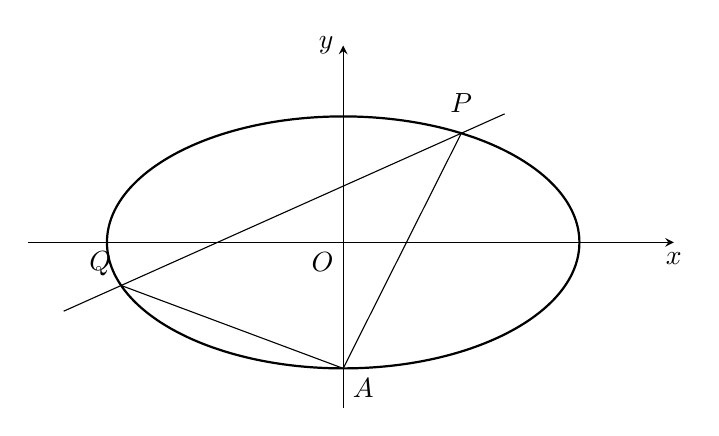
\begin{tikzpicture}[>=stealth,scale=1.0]
  % 坐标轴
  \draw[->] (-4.0,0)--(4.2,0) node[below] {$x$};
  \draw[->] (0,-2.1)--(0,2.5) node[left] {$y$};
  \node[below left] at (0,0) {$O$};
  % 椭圆
  \draw[thick] (0,0) ellipse (3 and 1.6);
  % 点 P、Q 与弦 PQ
  \coordinate (P) at (1.5,1.386);
  \coordinate (Q) at (-2.82,-0.547);
  \coordinate (A) at (0,-1.6);
  \draw (2.05,1.632)--(-3.55,-0.874);
  \draw (A)--(P);
  \draw (A)--(Q);
  \node[above=4pt] at (P) {$P$};
  \node[above left] at (Q) {$Q$};
  \node[below right] at (A) {$A$};
\end{tikzpicture}
\end{center}
\nopagebreak[4]
\Needspace{4\baselineskip}
\textbf{解析}

\textbf{（1）} 椭圆过 $A(0,-1)$，故 $b=1$。

\Needspace{5\baselineskip}
离心率 $e=\dfrac{c}{a}=\dfrac{\sqrt{2}}{2}$，故 $c^{2}=\dfrac{1}{2}a^{2}$，从而

\nopagebreak[4]
\[
b^{2}=a^{2}-c^{2}=\frac{1}{2}a^{2}=1,
\]

得 $a^{2}=2$。

\Needspace{5\baselineskip}
所以椭圆 $E$ 的方程为

\nopagebreak[4]
\[
\frac{x^{2}}{2}+y^{2}=1.
\]

\Needspace{5\baselineskip}
\textbf{（2）} 直线过点 $(1,1)$、斜率为 $k$，方程为

\nopagebreak[4]
\[
y=k(x-1)+1=kx+(1-k).
\]

\Needspace{5\baselineskip}
代入椭圆方程 $x^{2}+2y^{2}=2$：

\nopagebreak[4]
\[
x^{2}+2\left[kx+(1-k)\right]^{2}=2,
\]

\Needspace{5\baselineskip}
整理得

\nopagebreak[4]
\[
(1+2k^{2})x^{2}+4k(1-k)x+2(1-k)^{2}-2=0.
\]

\Needspace{5\baselineskip}
设 $P(x_{1},y_{1})$，$Q(x_{2},y_{2})$，则

\nopagebreak[4]
\[
x_{1}+x_{2}=-\frac{4k(1-k)}{1+2k^{2}},\qquad x_{1}x_{2}=\frac{2k(k-2)}{1+2k^{2}}.
\]

\Needspace{5\baselineskip}
直线 $AP$ 的斜率为

\nopagebreak[4]
\[
k_{AP}=\frac{y_{1}+1}{x_{1}}=\frac{kx_{1}+(2-k)}{x_{1}}=k+\frac{2-k}{x_{1}},
\]

\Needspace{5\baselineskip}
同理 $k_{AQ}=k+\dfrac{2-k}{x_{2}}$。于是

\nopagebreak[4]
\[
k_{AP}+k_{AQ}=2k+(2-k)\left(\frac{1}{x_{1}}+\frac{1}{x_{2}}\right)
=2k+(2-k)\cdot\frac{x_{1}+x_{2}}{x_{1}x_{2}}.
\]

\Needspace{5\baselineskip}
代入韦达定理：

\nopagebreak[4]
\[
\frac{x_{1}+x_{2}}{x_{1}x_{2}}=\frac{-4k(1-k)}{2k(k-2)}=\frac{2(1-k)}{2-k},
\]

\Needspace{5\baselineskip}
故

\nopagebreak[4]
\[
k_{AP}+k_{AQ}=2k+(2-k)\cdot\frac{2(1-k)}{2-k}=2k+2(1-k)=2.
\]

\gkanswer{答案（1）：$\dfrac{x^{2}}{2}+y^{2}=1$。}

\gkanswer{答案（2）：证明见解析。}

\end{answer}
\begin{answer}
\gksolhead{21}{}

\textbf{题目}：

设 $f_{n}(x)=x+x^{2}+\cdots+x^{n}-1$，$x\ge 0$，$n\in\mathbf{N}$，$n\ge 2$．

（1） 求 $f_{n}'(2)$；

（2） 证明：$f_{n}(x)$ 在 $\left(0,\dfrac{2}{3}\right)$ 内有且仅有一个零点（记为 $a_{n}$），且 $0<a_{n}-\dfrac{1}{2}<\dfrac{1}{3}\left(\dfrac{2}{3}\right)^{n}$．

\Needspace{4\baselineskip}
\textbf{解析}

\Needspace{5\baselineskip}
\textbf{（1）} 逐项求导：

\nopagebreak[4]
\[
f_{n}'(x)=1+2x+3x^{2}+\cdots+nx^{n-1}.
\]

\Needspace{5\baselineskip}
代入 $x=2$：

\nopagebreak[4]
\[
f_{n}'(2)=1+2\cdot 2+3\cdot 2^{2}+\cdots+n\cdot 2^{n-1}.
\]

\Needspace{5\baselineskip}
由错位相减（或公式 $\displaystyle\sum_{k=1}^{n}k\cdot 2^{k-1}=1+(n-1)2^{n}$）得

\nopagebreak[4]
\[
f_{n}'(2)=(n-1)2^{n}+1.
\]

\textbf{（2）} 当 $x>0$ 时 $f_{n}'(x)=1+2x+\cdots+nx^{n-1}>0$，故 $f_{n}$ 在 $[0,+\infty)$ 上严格递增，零点至多一个。

\Needspace{5\baselineskip}
计算端点附近的函数值。由等比数列求和，

\nopagebreak[4]
\[
f_{n}\left(\frac{1}{2}\right)=\frac{\frac{1}{2}\left(1-\frac{1}{2^{n}}\right)}{1-\frac{1}{2}}-1=1-\frac{1}{2^{n}}-1=-\frac{1}{2^{n}}<0,
\]

\nopagebreak[4]
\[
f_{n}\left(\frac{2}{3}\right)=\frac{\frac{2}{3}\left(1-\left(\frac{2}{3}\right)^{n}\right)}{1-\frac{2}{3}}-1=1-2\left(\frac{2}{3}\right)^{n}.
\]

当 $n\ge 2$ 时 $2\left(\dfrac{2}{3}\right)^{n}\le 2\cdot\dfrac{4}{9}=\dfrac{8}{9}<1$，故 $f_{n}\left(\dfrac{2}{3}\right)>0$。

\Needspace{5\baselineskip}
由零点存在定理及单调性，$f_{n}$ 在 $\left(0,\dfrac{2}{3}\right)$ 内有且仅有一个零点 $a_{n}$，且由 $f_{n}\left(\dfrac{1}{2}\right)<0$ 得

\nopagebreak[4]
\[
a_{n}>\frac{1}{2}.
\]

\Needspace{5\baselineskip}
由 $f_{n}(a_{n})=0$ 得 $a_{n}+a_{n}^{2}+\cdots+a_{n}^{n}=1$，即

\nopagebreak[4]
\[
\frac{a_{n}\left(1-a_{n}^{n}\right)}{1-a_{n}}=1.
\]

\Needspace{5\baselineskip}
去分母整理：

\nopagebreak[4]
\[
a_{n}-a_{n}^{n+1}=1-a_{n},
\]

\Needspace{5\baselineskip}
即

\nopagebreak[4]
\[
2a_{n}-1=a_{n}^{n+1},\qquad a_{n}-\frac{1}{2}=\frac{a_{n}^{n+1}}{2}.
\]

因 $a_{n}>\dfrac{1}{2}>0$，右端为正，故 $a_{n}-\dfrac{1}{2}>0$。

\Needspace{5\baselineskip}
又 $a_{n}<\dfrac{2}{3}$，故

\nopagebreak[4]
\[
a_{n}-\frac{1}{2}=\frac{a_{n}^{n+1}}{2}<\frac{1}{2}\left(\frac{2}{3}\right)^{n+1}=\frac{1}{3}\left(\frac{2}{3}\right)^{n}.
\]

\Needspace{5\baselineskip}
综上，

\nopagebreak[4]
\[
0<a_{n}-\frac{1}{2}<\frac{1}{3}\left(\frac{2}{3}\right)^{n}.
\]

\gkanswer{答案（1）：$f_{n}'(2)=(n-1)2^{n}+1$。}

\gkanswer{答案（2）：证明见解析。}

\end{answer}
\begin{answer}
\gksolhead{22}{}

\textbf{题目}：

如图，$AB$ 切 $\odot O$ 于点 $B$，直线 $AO$ 交 $\odot O$ 于 $D$，$E$ 两点，$BC\perp DE$，垂足为 $C$．

（1） 证明：$\angle CBD=\angle DBA$；

（2） 若 $AD=3DC$，$BC=\sqrt{2}$，求 $\odot O$ 的直径．
\nopagebreak[4]
\begin{center}% 2015 年陕西卷（文史类）第 22 题：圆的切线与割线（依固定扫描页重绘，只画拓扑与标号，不按比例）
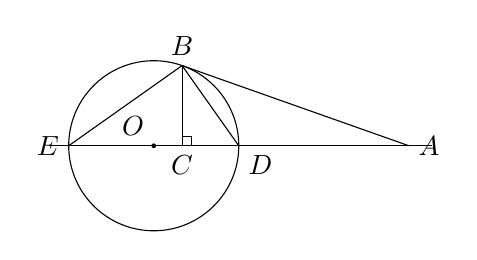
\begin{tikzpicture}[>=stealth,scale=0.72]
  % 圆 O
  \draw (0,0) circle (1.5);
  \fill (0,0) circle (1.2pt);
  \node[above left] at (0,0) {$O$};
  % 割线 A-D-C-O-E
  \draw (-1.85,0)--(4.9,0);
  \coordinate (E) at (-1.5,0);
  \coordinate (C) at (0.5,0);
  \coordinate (D) at (1.5,0);
  \coordinate (A) at (4.5,0);
  \coordinate (B) at (0.5,1.414);
  % 切线与弦
  \draw (B)--(A);
  \draw (B)--(E);
  \draw (B)--(D);
  \draw (B)--(C);
  % 直角标记
  \draw (0.5,0.16)--(0.66,0.16)--(0.66,0);
  % 标号
  \node[above] at (B) {$B$};
  \node[left] at (E) {$E$};
  \node[below] at (C) {$C$};
  \node[below right] at (D) {$D$};
  \node[right] at (A) {$A$};
\end{tikzpicture}
\end{center}
\nopagebreak[4]
\Needspace{4\baselineskip}
\textbf{解析}

\Needspace{5\baselineskip}
\textbf{（1）} 因 $AB$ 切 $\odot O$ 于 $B$，故 $OB\perp AB$，即 $\angle OBA=90^{\circ}$，于是

\nopagebreak[4]
\[
\angle DBA=90^{\circ}-\angle OBD.
\]

\Needspace{5\baselineskip}
又 $BC\perp DE$，垂足为 $C$，在直角三角形 $BCD$ 中

\nopagebreak[4]
\[
\angle CBD=90^{\circ}-\angle BDC.
\]

因 $D$，$O$，$E$ 共线，$\angle BDC=\angle BDO$；又 $OB=OD$，三角形 $OBD$ 为等腰三角形，$\angle OBD=\angle BDO$。

\Needspace{5\baselineskip}
故

\nopagebreak[4]
\[
\angle CBD=90^{\circ}-\angle OBD=\angle DBA.
\]

\Needspace{5\baselineskip}
\textbf{（2）} 设 $\odot O$ 半径为 $r$，$OC=x$。由 $O$，$C$，$D$ 依次共线得 $DC=r-x$，而 $OD=r$，故

\nopagebreak[4]
\[
OA=OD+DA=r+3(r-x)=4r-3x.
\]

\Needspace{5\baselineskip}
因 $OB\perp AB$，$BC$ 是直角三角形 $OBA$ 斜边 $OA$ 上的高，由射影定理

\nopagebreak[4]
\[
OB^{2}=OC\cdot OA,\qquad BC^{2}=OC\cdot CA.
\]

\Needspace{5\baselineskip}
第一式给出

\nopagebreak[4]
\[
r^{2}=x(4r-3x),
\]

即 $r^{2}-4rx+3x^{2}=0$，分解得 $(r-x)(r-3x)=0$。因 $D$ 与 $C$ 不重合，$r\ne x$，故 $r=3x$。

\Needspace{5\baselineskip}
第二式中 $CA=OA-OC=4r-4x$，代入 $BC=\sqrt{2}$：

\nopagebreak[4]
\[
2=4x(r-x)=4x\cdot 2x=8x^{2},
\]

得 $x=\dfrac{1}{2}$，从而 $r=\dfrac{3}{2}$。

所以 $\odot O$ 的直径为 $2r=3$。

\gkanswer{答案（1）：证明见解析。}

\gkanswer{答案（2）：$\odot O$ 的直径为 $3$。}

\end{answer}
\begin{answer}
\gksolhead{23}{}

\textbf{题目}：

在直角坐标系 $xOy$ 中，直线 $l$ 的参数方程为 $\begin{cases}x=3+\dfrac{1}{2}t,\\[4pt] y=\dfrac{\sqrt{3}}{2}t,\end{cases}$（$t$ 为参数），以原点为极点，$x$ 轴正半轴为极轴建立极坐标系，$\odot C$ 的极坐标方程为 $\rho=2\sqrt{3}\sin\theta$．

（1） 写出 $\odot C$ 的直角坐标方程；

（2） $P$ 为直线 $l$ 上一动点，当 $P$ 到圆心 $C$ 的距离最小时，求 $P$ 的直角坐标．

\Needspace{4\baselineskip}
\textbf{解析}

\Needspace{5\baselineskip}
\textbf{（1）} 由 $\rho=2\sqrt{3}\sin\theta$ 得 $\rho^{2}=2\sqrt{3}\rho\sin\theta$。用 $\rho^{2}=x^{2}+y^{2}$，$\rho\sin\theta=y$ 代换：

\nopagebreak[4]
\[
x^{2}+y^{2}=2\sqrt{3}y,
\]

\Needspace{5\baselineskip}
配方得

\nopagebreak[4]
\[
x^{2}+(y-\sqrt{3})^{2}=3.
\]

\Needspace{5\baselineskip}
\textbf{（2）} 由参数方程消去 $t$：$\dfrac{x-3}{1/2}=\dfrac{y}{\sqrt{3}/2}$，即

\nopagebreak[4]
\[
y=\sqrt{3}(x-3).
\]

圆心为 $C(0,\sqrt{3})$。点 $P$ 到 $C$ 的距离最小时，$CP\perp l$，$P$ 是 $C$ 在 $l$ 上的投影。

\Needspace{5\baselineskip}
直线 $l$ 的一般式为 $\sqrt{3}x-y-3\sqrt{3}=0$，点 $C$ 到 $l$ 的距离为

\nopagebreak[4]
\[
d=\frac{|\sqrt{3}\cdot 0-\sqrt{3}-3\sqrt{3}|}{\sqrt{3+1}}=\frac{4\sqrt{3}}{2}=2\sqrt{3}.
\]

\Needspace{5\baselineskip}
$l$ 的单位法向量为 $\left(\dfrac{\sqrt{3}}{2},-\dfrac{1}{2}\right)$，且 $C$ 代入一般式左端为负，故投影为

\nopagebreak[4]
\[
P=C+2\sqrt{3}\left(\frac{\sqrt{3}}{2},-\frac{1}{2}\right)=(0,\sqrt{3})+(3,-\sqrt{3})=(3,0).
\]

\gkanswer{答案（1）：$x^{2}+(y-\sqrt{3})^{2}=3$。}

\gkanswer{答案（2）：$P(3,0)$。}

\end{answer}
\begin{answer}
\gksolhead{24}{}

\textbf{题目}：

已知关于 $x$ 的不等式 $|x+a|<b$ 的解集为 $\{x\mid 2<x<4\}$．

（1） 求实数 $a$，$b$ 的值；

（2） 求 $\sqrt{at+12}+\sqrt{bt}$ 的最大值．

\Needspace{4\baselineskip}
\textbf{解析}

\Needspace{5\baselineskip}
\textbf{（1）} 由 $|x+a|<b$（$b>0$）得

\nopagebreak[4]
\[
-b<x+a<b,\qquad -a-b<x<-a+b.
\]

\Needspace{5\baselineskip}
解集为 $(2,4)$，故

\nopagebreak[4]
\[
-a-b=2,\qquad -a+b=4.
\]

两式相加得 $-2a=6$，即 $a=-3$；两式相减得 $2b=2$，即 $b=1$。

\Needspace{5\baselineskip}
\textbf{（2）} 代入 $a=-3$，$b=1$：

\nopagebreak[4]
\[
\sqrt{at+12}+\sqrt{bt}=\sqrt{12-3t}+\sqrt{t}.
\]

\Needspace{5\baselineskip}
由柯西不等式，

\nopagebreak[4]
\[
\left(\sqrt{12-3t}+\sqrt{t}\right)^{2}\le (3+1)\left[(4-t)+t\right]=16,
\]

\Needspace{5\baselineskip}
故

\nopagebreak[4]
\[
\sqrt{12-3t}+\sqrt{t}\le 4.
\]

等号成立当且仅当 $\dfrac{4-t}{3}=t$，即 $t=1$，此时两根式分别为 $3$ 与 $1$，在定义域 $0\le t\le 4$ 内。

所以最大值为 $4$。

\gkanswer{答案（1）：$a=-3$，$b=1$。}

\gkanswer{答案（2）：最大值为 $4$。}

\end{answer}